
\subsection{Algoritmos}
	\label{subsec:principaisalgoritimos}
% Lembrando que tem muuuuitos outros. Principalmente os baseados em tópicos. -- Rafael % -? antes falar das técnicas (janelas, agrupamento, tópicos, etc..) ?
% falar um pouco sobre TT e C99, sobre como foram pioneiros, influenciáram muitos outros e são empregrados até hoje;
% Nem mencionou janelas deslizantes anteriormente. --> Rafael
% -? Criar um texto sobre janelas deslizantes?
% \textit{threshold}. %TODO - explicar como se encontra os vales


% ==========  TextTiling  ==========

Entre os trabalhos tradicionais da literatura podemos citar o  \textit{TextTiling}~\cite{Hearst1994} e o \textit{C99}~\cite{Choi2000}.
% TT pioneiro e simples, mas pouco acurado
% C99 utiliz




O \textit{TextTiling} é um algoritmo baseado em janelas deslizantes, em  que, para cada candidato a limite, analisa-se o texto circundante. Um limite ou quebra entre segmentos é identificado sempre que a similaridade entre as unidades que antecedem e precedem o ponto candidato cai abaixo de um limiar. O \textit{TextTiling} recebe uma lista de candidatos a limite, usualmente finais de parágrafo ou finais de sentenças. Para cada posição candidata são construídos 2 blocos, um contendo sentenças que a precedem e outro com as que a sucedem. O tamanho desses blocos é um parâmetro a ser fornecido ao algoritmo e determina o tamanho mínimo de um segmento. Em seguida, os blocos de texto são representados por vetores que contém as frequências de suas palavras. Então, usa-se cosseno (Equação~\ref{equ:cosine}) para calcular a similaridade entre os blocos adjacentes a cada candidato e identifica-se uma transição entre tópicos pelos vales na curva de dissimilaridade.
% Rafael --> Podem ter vários tipos de cursa. Ser mais objetivo. Quando a similaridade fica abaixo de um limiar fornecido pelo usuário.? Na verdade, dá pra fazer uma mescla. 
%TODO como apresentado na Figura~\ref{fig:curvadedissimilaridade}.

O \textit{TextTiling} possui baixa complexidade computacional. Por outro lado, algoritmos mais complexos, como os baseados em matrizes de similaridade, apresentam acurácia relativamente superior como apresentado em~\cite{Choi2000, Kern2009, Misra2009}.




% ==========  C99  ==========

Outro algoritmo frequentemente referenciado na literatura é o C99 o qual é baseado em \textit{ranking}. Embora muitos trabalhos utilizem matrizes de similaridades para pequenos segmentos, o cálculo de suas similaridades não é confiável, pois uma ocorrência adicional de uma palavra pode causar certo impacto e alterar o cálculo da similaridade~\cite{Choi2000}. Além disso, o estilo da escrita normalmente não ser constante em todo o texto. Por exemplo, textos iniciais dedicados a introdução costumam apresentar menor coesão do que trechos dedicados a um tópico específico. Portanto, comparar a similaridade entre trechos de diferentes regiões não é apropriado. Devido a isso, as similaridades não podem ser comparadas em valores absolutos. Então, contorna-se esse problema fazendo uso de \textit{rankings} de similaridade para encontrar os segmentos de texto. Para isso, o C99 constrói uma matriz que contém as similaridades de todas as unidades de informação (normalmente sentenças ou parágrafos). Em seguida, cada valor na matriz de similaridade é substituído por seu \textit{ranking local}. Para cada elemento da matriz, seu \textit{ranking} é o número de elementos vizinhos com valor de similaridade menor que o seu. Então, cada elemento e comparado com seus vizinhos dentro de uma região denominada máscara.

Na Figura~\ref{fig:a} é destacado um quadro 3~x~3 de uma matriz em que cada elemento é a similaridade entre duas unidades de informação. Tomando como exemplo o elemento com valor $0,5$, a mesma posição na matriz de \textit{rankings} terá o valor $4$, pois esse é o número de vizinhos com valores inferiores a $0,5$ dentro do quadro analisado na matriz de similaridades. Da mesma forma, na Figura~\ref{fig:b} para o valor $0,2$ a matriz de \textit{rankings} conterá o valor $1$ na mesma posição.

\begin{figure}[!h]
	\centering     %%% not \center

	\subfigure[Passo 1]{\label{fig:a}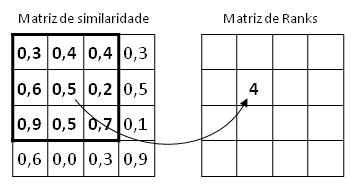
\includegraphics[width=60mm]{conteudo/capitulos/figs/exemplo-matrix-rank-A.png}}
	\subfigure[Passo 2]{\label{fig:b}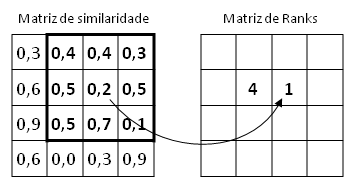
\includegraphics[width=60mm]{conteudo/capitulos/figs/exemplo-matrix-rank-B.png}}
	
	\caption{Exemplo de construção de uma matriz de rankings.%~\cite{Choi2000}.
	}
	\label{fig:exemplomatrixrank}
\end{figure}
% -< Colocar uma explicação mais detalhada para esses passos



Finalmente, com base na matriz de \textit{ranking}, o C99 utiliza um método de \textit{clustering} baseado no algoritmo de maximização de Reynar para identificar os limites entre os segmentos. 
% ~\cite{Reynar1998} 
% Rafael: Esse passo aqui tá meio obscuro ainda. Não dá pra fazer uma figura ilustrativa?






% ==========  Utiyama  ==========





% ==========  BayesSeg  ==========



Os métodos baseados em coesão léxica que utilizam métricas como cosseno quantificam a similaridade entre sentenças baseando-se apenas na frequência das palavras, Essa abordagem, ignora certas características do texto que podem dar pistas sobre a estrutura do texto. Por exemplo, frases como "Prosseguindo", "Dando continuidade", "Ao final da reunião" podem dar "pistas" de inicio ou final de segmento. A fim de aproveitar esses indicadores, usa-se um framework bayesiano que permite incorporar fontes externas ao modelo. O método BayesSeg~\cite{Eisenstein2008} aborda a coesão léxica em um contexto bayesiano onde as palavas de um segmento surgem de um modelo de linguagem multinomial o qual é associado a um assunto. 

Essa abordagem é similar à métodos probabilísticos de extração de tópicos como o Latent Dirichlet Allocation (LDA)~\cite{Blei2003}, com a diferença que ao invés de atribuir tópicos ocultos a cada palavra, esses são usados para segmentar o documento. Nesse sentido, detecta-se um limite entre sentenças quando a distribuição de tópicos entre elas for diferente.

Baseia-se na ideia que alguns termos são usados em tópicos específicos enquanto outros são neutros em relação aos tópicos do documento e são usados para expressar uma estrutura do documento, ou seja, as "frases-pista" vem de um único modelo generativo. A fim de refletir essa ideia, o modelo é adaptado para influenciar a probabilidade da sentença de ser uma final ou início de segmento conforme a presença de "frases pista".











